\section{Sch\"{a}r mountain waves}
\label{sec:slanted:schaerWaves}

\TODO{
\begin{itemize}
	\item Meshes: BTF, cut cell, slanted cell, SLEVE?
	\item Conclusion: linearUpwind solution similar to non-cancellation of metric terms in \citep{klemp2003}
	\item Conclusion: unlike linearUpwind, cubicFit gives the correct solution (at least on BTF? is linearUpwind better on cut/slanted cells?)
	\item Conclusion: cubicFit produces almost identical results on BTF, cut cell and slanted cell meshes.  Unlike the results in \citep{shaw-weller2016}, errors in potential temperature are negligible using the cubicFit scheme.
	\item Conclusion: should we test max(dt) again? we've not yet done so for a dynamical test.  I'd hope that slanted cells are much better than cut cells.
\end{itemize}
}

The test originally specified by \citet{schaer2002} prescribes flow over terrain with small-scale and large-scale undulations which induces propagating and evanescent gravity waves.  \TODO{what is the motivation for this test?  it is needed to assess the dynamics solver with horizontal and vertical transport}

Following \citet{melvin2010}, the domain is \SI{300}{\kilo\meter} wide and \SI{30}{\kilo\meter} high, and the mesh spacing is $\Delta x = \SI{500}{\meter}$ and $\Delta z^\star = \SI{300}{\meter}$.
The mountain profile has the same form as equation~\eqref{eqn:resting:mountain}, but the mountain waves test has a lower peak mountain height of $h_0 = \SI{250}{\meter}$.  As in the resting atmosphere test, $a = \SI{5}{\kilo\meter}$ is the mountain half-width and $\lambda = \SI{4}{\kilo\meter}$ is the wavelength.

A uniform horizontal wind $(u, w) = (10, 0)\:\si{\meter\per\second}$ is prescribed in the interior domain and at the inlet boundary.  No normal flow is imposed at the top and bottom boundaries and the velocity field has a zero gradient outlet boundary condition.

The initial thermodynamic conditions have constant static stability with $N = \SI{0.01}{\per\second}$ everywhere such that
\begin{align}
	\theta(z) = \theta_0 \exp \left( \frac{N^2}{g} z \right) \label{eqn:slanted:schaerWaves:thermal-profile}
\end{align}
where the temperature at $z=0$ is $\theta_0 = \SI{288}{\kelvin}$.
Potential temperature values are prescribed at the inlet and upper boundary using equation~\eqref{eqn:slanted:schaerWaves:thermal-profile}, and a zero gradient boundary condition is applied at the outlet.
At the ground, fixed gradients are imposed by calculating the component of $\nabla \theta$ normal to each face using the vertical derivative of equation~\eqref{eqn:slanted:schaerWaves:thermal-profile}.
For the Exner function of pressure, hydrostatic balance is prescribed on top and bottom boundaries and the inlet and outlet are zero normal gradient.

Sponge layers are added to the upper \SI{10}{\kilo\meter} and leftmost \SI{10}{\kilo\meter} at the inlet boundary to damp the reflection of waves.
The damping function, \(\mu\), is adapted from \citet{melvin2010} such that
\begin{align}
	\mu(x, z) &= \mu_\mathrm{upper} + \mu_\mathrm{inlet} \\
	\mu_\mathrm{upper}(z) &= \begin{cases}
		\overline{\mu} \sin^2 \left( \frac{\pi}{2} \frac{z - z_B}{H - z_B} \right) & \text{if } z \geq z_B \\
		0 & \text{otherwise} \\
	\end{cases} \\
	\mu_\mathrm{inlet}(x) &= \begin{cases}
		\overline{\mu} \sin^2 \left( \frac{\pi}{2} \frac{x_I - x}{x_I - x_0} \right) & \text{if } x < x_I \\
		0 & \text{otherwise}
	\end{cases}
\end{align}
where $\overline{\mu} = \SI{1.2}{\per\second}$ is the damping coefficient, $z_B = \SI{20}{\kilo\meter}$ is the bottom of the sponge layer, $H = \SI{30}{\kilo\meter}$ is the top of the domain, $x_0 = \SI{-150}{\kilo\meter}$ is the leftmost limit of the domain and $x_I = \SI{-140}{\kilo\meter}$ is the rightmost extent of the inlet sponge layer.  The sponge layer is only active on faces whose normal is vertical so that it damps vertical momentum only.
Note that, while the domain itself is \SI{30}{\kilo\meter} in height, for the purposes of generating BTF meshes, the domain height is set to \SI{20}{\kilo\meter} because the sponge layer occupies the uppermost \SI{10}{\kilo\meter}.

\begin{figure}
	\centering
	\begin{subfigure}{0.55\textwidth}
		\centering
		\caption{Lorenz staggering, linearUpwind transport}
		\label{fig:slanted:schaerWaves:w:linearUpwind}
		\includegraphics{thesis/slanted/schaerWaves/fig-btf-300dz-linearUpwind-w.pdf}
	\end{subfigure}
	\begin{subfigure}{0.44\textwidth}
		\centering
		\caption{Lorenz staggering, cubicFit transport}
		\label{fig:slanted:schaerWaves:w:cubicFit}
		\includegraphics{thesis/slanted/schaerWaves/fig-btf-300dz-cubicFit-w.pdf}
	\end{subfigure}
	\\
	\vspace*{1em}
	%
	\begin{subfigure}{0.55\textwidth}
		\centering
		\caption{Charney--Phillips staggering}
		\label{fig:slanted:schaerWaves:w:cp}
		\includegraphics{thesis/slanted/schaerWaves/fig-btf-300dz-cp-w.pdf}
	\end{subfigure}
	\begin{subfigure}{0.44\textwidth}
		\centering
		\caption{Reference solution by \citet{melvin2010}}
		\label{fig:slanted:schaerWaves:w:melvin}
		\raisebox{0.2in}{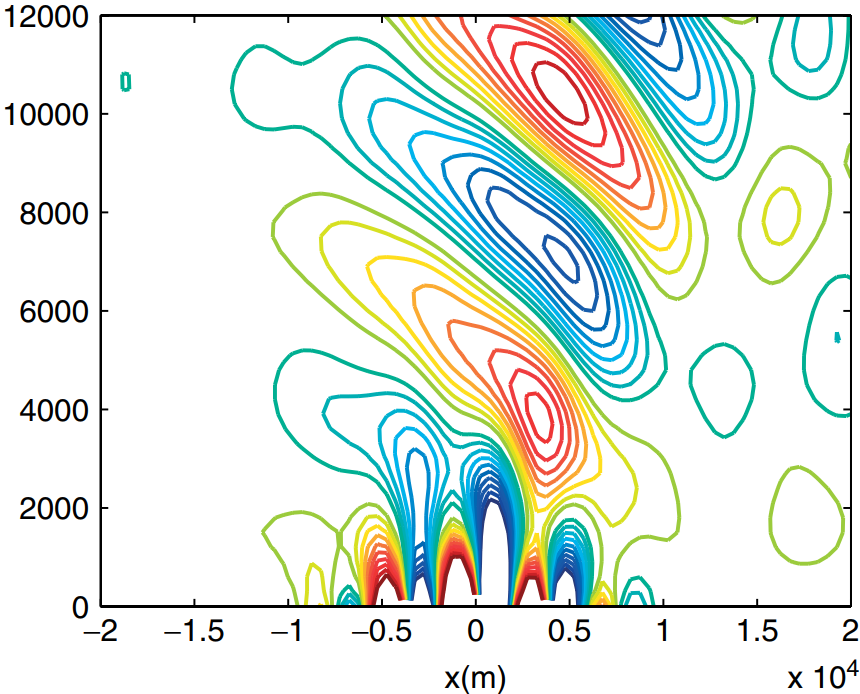
\includegraphics[height=1.9in]{slanted/schaerWaves/melvin2010-w-mass-conserving-sisl.png}}
	\end{subfigure}
	\caption{Vertical velocities at the end of integration of the Sch\"{a}r mountain waves test case.
	Results obtained using a BTF mesh and Lorenz staggering, with potential temperature and momentum transported by (\subcaptionref{fig:slanted:schaerWaves:w:linearUpwind}) the linearUpwind scheme and
	(\subcaptionref{fig:slanted:schaerWaves:w:cubicFit}) the cubicFit scheme, and (\subcaptionref{fig:slanted:schaerWaves:w:cp}) using a BTF mesh and Charney--Phillips staggering.
	For comparison, (\subcaptionref{fig:slanted:schaerWaves:w:melvin}) provides a reference solution obtained with a mass-conserving semi-implicit semi-Lagrangian model \citep{melvin2010}.
	Contours are plotted every \SI{0.05}{\meter\per\second}.  In figures (\subcaptionref{fig:slanted:schaerWaves:w:linearUpwind}), (\subcaptionref{fig:slanted:schaerWaves:w:cubicFit}) and (\subcaptionref{fig:slanted:schaerWaves:w:cp}), ascending velocities are marked by solid black lines and descending velocities are marked by dashed red lines.}
	\label{fig:slanted:schaerWaves:w}
\end{figure}

